\documentclass[journal]{IEEEtran}
\usepackage[utf8]{inputenc}
\usepackage{graphicx}
\usepackage[hyphens]{url}

\title{An FPGA Implementation of a \\ Digital Storage Oscilloscope}
\author{Andrei~Purcarus,~\IEEEmembership{McGill~University} and Ze~Yu~Yang,~\IEEEmembership{McGill~University}}

\begin{document}
\sloppy

\maketitle

\begin{abstract}

This paper discusses the implementation of a digital storage oscilloscope on the DE1-SoC Cyclone V FPGA development board. This oscilloscope is capable of displaying the sample points captured by an ADC on a VGA monitor. It is also capable of measuring the frequency of waveforms with at most 0.10\% error over a range of frequencies from 1kHz to 200kHz. Due to the lack of interpolation and voltage measurement modules, the oscilloscope has yet to be fully evaluated. In addition, the performance of the oscilloscope has only been tested for simulated digital waveforms, and has yet to be characterized against real analog waveforms.

\end{abstract}

\begin{IEEEkeywords}

Digital storage oscilloscope, FPGA, real-time processing, sin(x)/x interpolation.

\end{IEEEkeywords}

\section{Introduction}

The purpose of this project is to implement the digital components of a digital storage oscilloscope (DSO) on an FPGA device. We will assume that the analog input circuitry is already available, with the processed analog signal having been converted to a digital signal through an ADC. We will target the Cyclone V DE1-SoC FPGA development board, which contains a 50~MHz base clock, a 12-bit, 500~kSa/s ADC and a 24-bit video DAC connected to a VGA D-Sub connector \cite{DE1SoC,ltc2308}. Hence, the DSO will process digital signals coming from the ADC and display the resulting waveforms on a VGA monitor.

This project is motivated by the fact that traditional DSOs use a microprocessor to perform their processing, and this tends to be a bottleneck for real-time processing and complex operations such as the FFT \cite{tektronix_xyz_2016}. We aim to eliminate this bottleneck by providing a pipelined, parallel implementation of the DSO functionality.

This functionality consists of capturing waveform data to an internal memory, and displaying the data when triggered by a predefined event. This event usually consists of the input waveform crossing a certain reference level with a positive or negative slope, referred to as rising edge and falling edge triggering, respectively \cite{tektronix_xyz_2016}. It is necessary to have this trigger for a stable waveform display, as it centers a periodic waveform on the same point over multiple video frames.

Although DSOs have been implemented on FPGAs before as student projects, the lack of proper interpolation led to a maximum displayable waveform frequency of 30~kHz using the same development board \cite{jin_digital_2016}. We aim to do better by using sin(x)/x interpolation techniques on the captured waveforms, which will allow us to perfectly reconstruct band-limited signals of frequencies less than 250~kHz, as given by the Nyquist criterion and our ADC sample rate. This is done by inserting zeros in between sample points (up-sampling), and applying a low-pass filter on the resulting waveform, which results in a perfect reconstruction of the waveform at the up-sampled points \cite{rehorn_sin_2009}.

For our design, we will aim for a maximum frequency of 200~kHz. This frequency was chosen to account for practical limitations in the interpolation algorithm. Since an ideal low-pass filter is impossible to achieve in practice, we will use a FIR filter with a finite roll-off. To avoid aliasing and ensure sufficient attenuation in the stop-band, we thus chose a lower cutoff frequency.

We will also aim for a minimum frequency of 1~kHz, which was chosen for simplicity as an order of magnitude higher than typical VGA frame rates of 60~Hz to 72~Hz \cite{vga_timing}. This will allow for multiple waveform captures over a single frame, and hence allow us to perform processing in real time.

In addition, although we will not be measuring the waveform frequency explicitly, we will measure the frequency at which the oscilloscope is triggered. This serves as a proxy for the waveform frequency, and will correctly identify it for waveforms with one trigger per period, such as sine and square waves. We will compare the accuracy of this measurement to the frequency measurement accuracy obtained by previous projects \cite{jin_digital_2016}. The resolution of our frequency measurement will be limited by the clock rate, and we will therefore aim for an accuracy of 1~\%~+~10~Hz over a frequency range of 1~kHz to 200~kHz.

Finally, we will perform voltage measurements on the captured waveform data, and output these to the display. We aim to produce peak-peak, average, max and min voltage measurements for the captured waveforms. Given that we have a 12-bit ADC with a range of 0.000~V to 4.095~V, we will aim for an accuracy of 1~\%~+~10 mV on these measurements over the entire frequency range. It is here that interpolation will really be tested since for higher frequencies the limited sampling rate means that we might not be able to capture the peaks of the waveform through the ADC. Hence we will rely on interpolation to produce these values, and compare them to the actual values.

For evaluation, the project will first be simulated using a frequency synthesizer and analog waveform generator designed in a previous assignment for this course. The VGA output signals will be logged to a text file, and this text file will be used to view the VGA display using a simulator \cite{vga_sim}. Then, the project will be synthesized on the FPGA board and analog signals from a signal generator will be fed to the ADC and compared to the readouts on a commercial DSO.

\section{Design Methodology}

\begin{figure}[!htb]
  \centering
  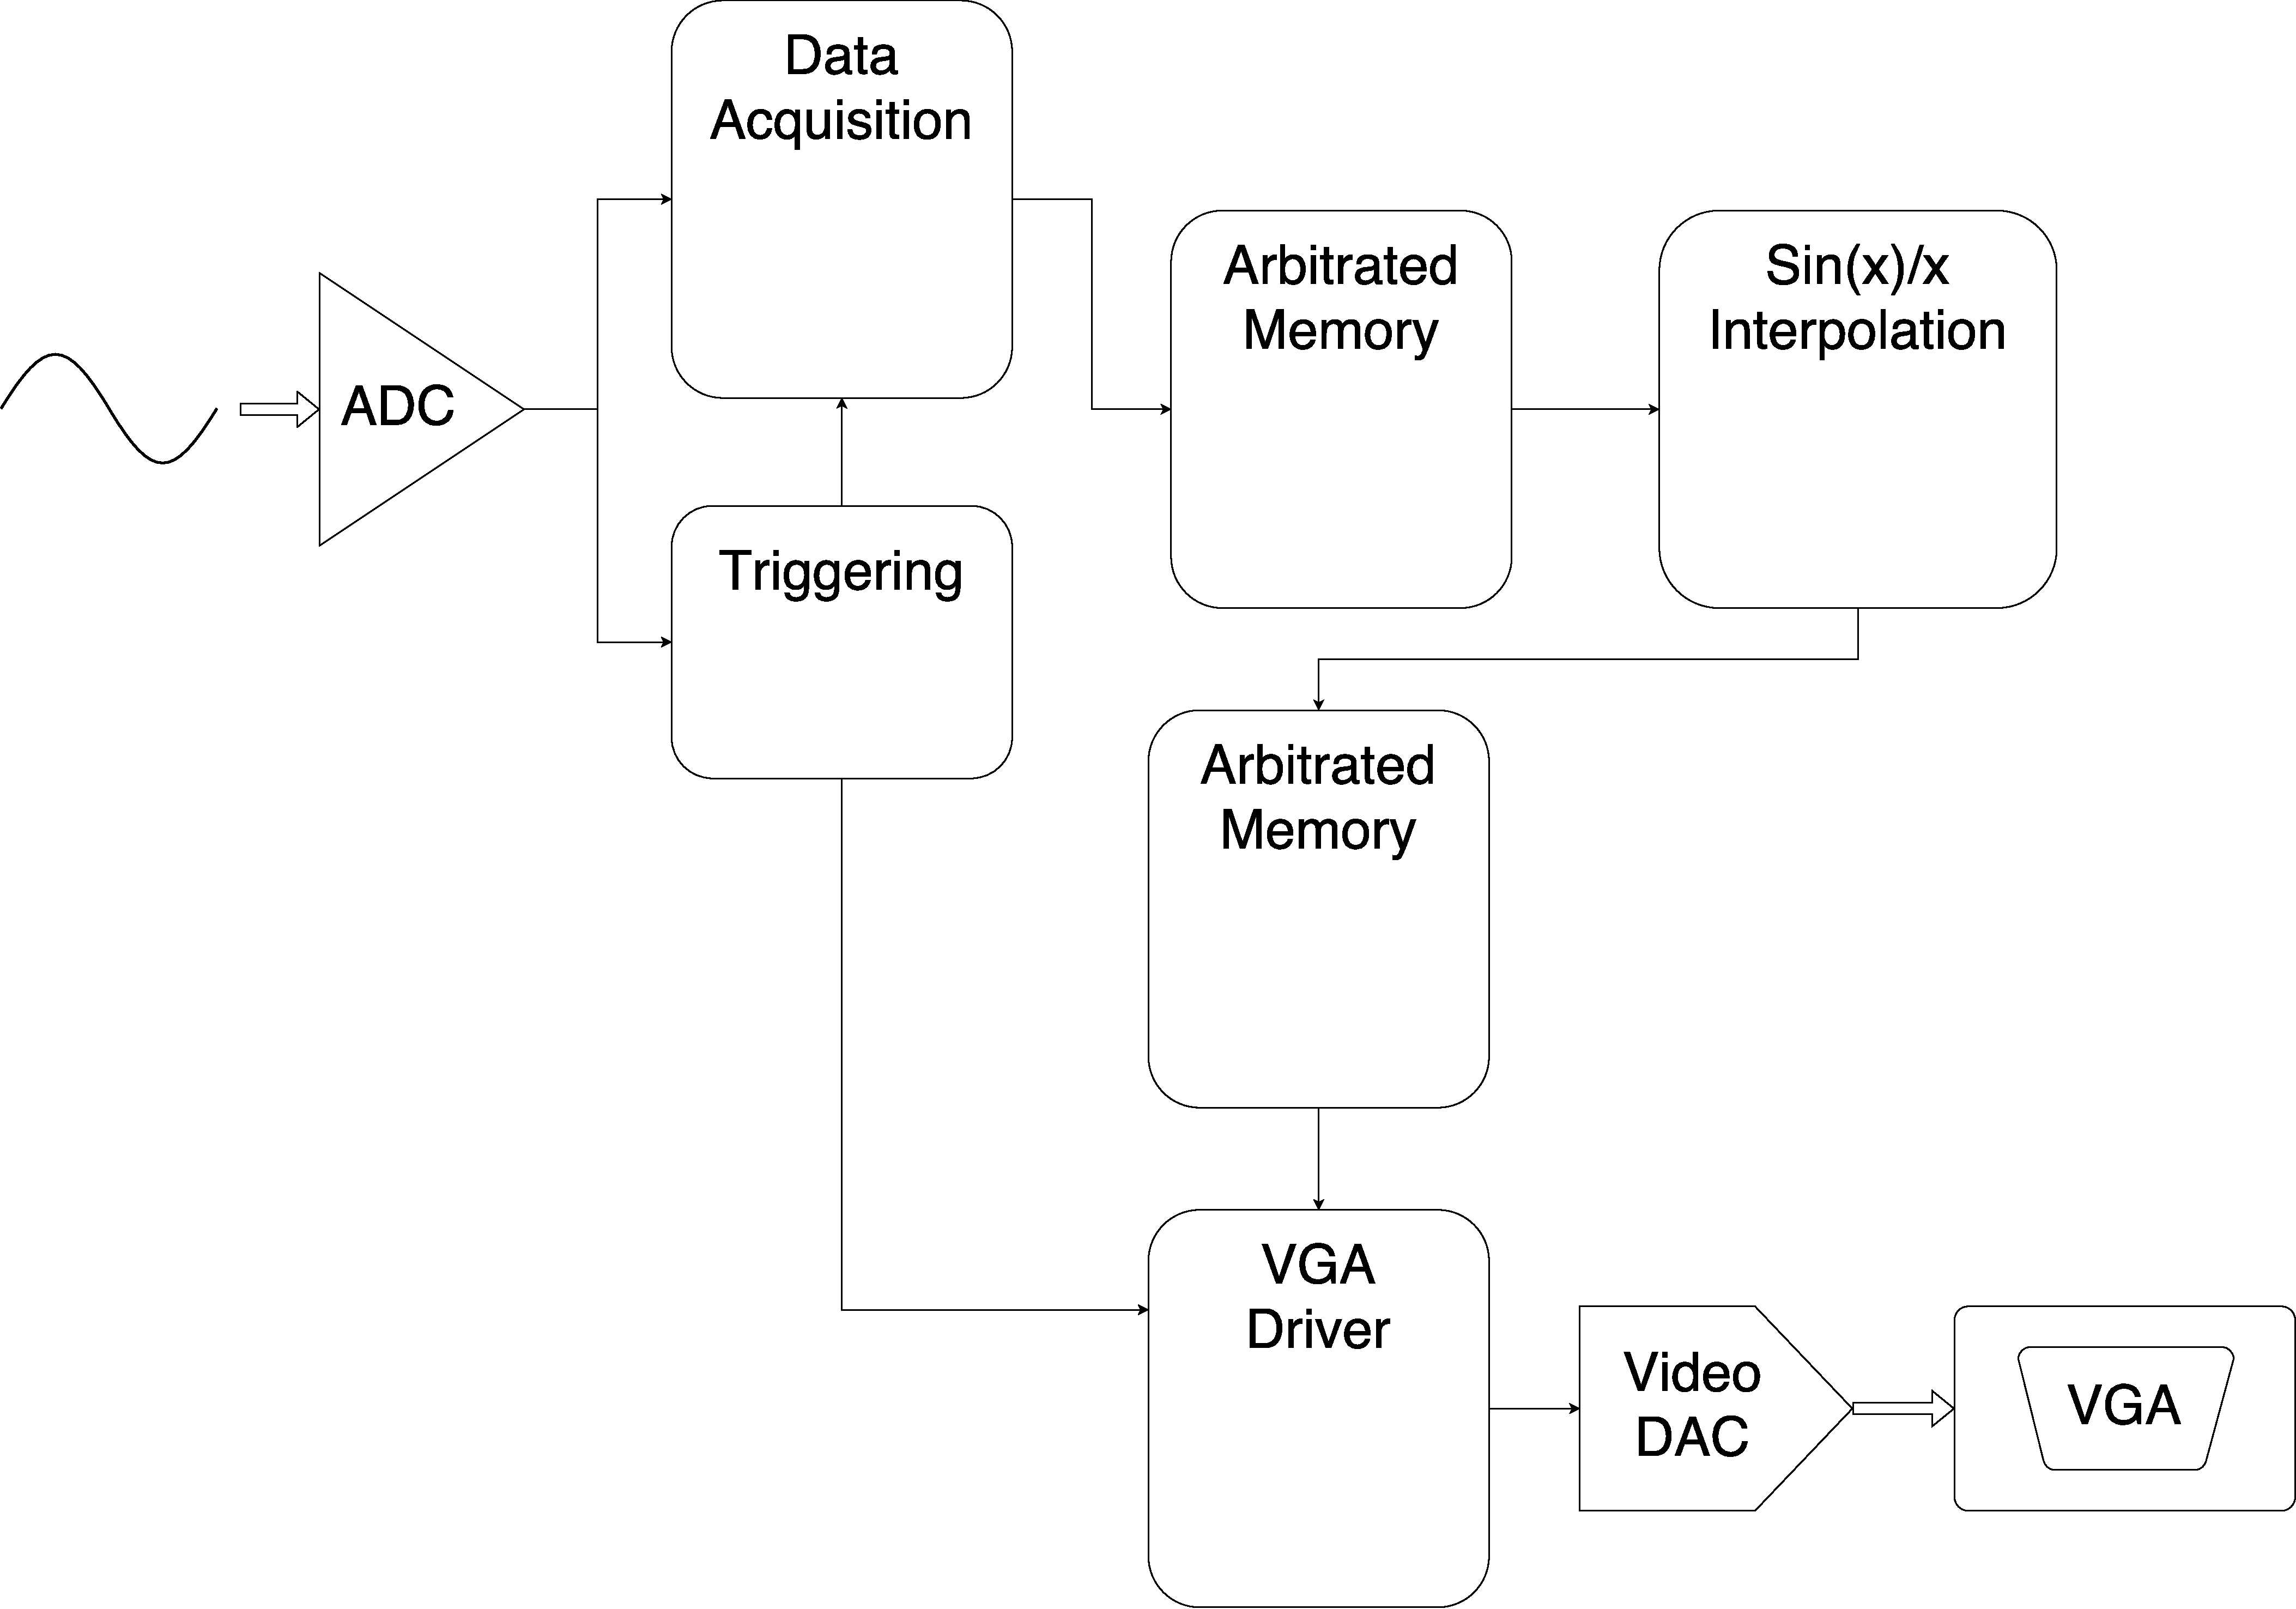
\includegraphics[width=\columnwidth]{diagrams/system.pdf}
  \caption{Simplified top-level block diagram of the DSO.}
  \label{fig:system}
\end{figure}

A simplified block diagram of the DSO is shown in Figure~\ref{fig:system}. The analog waveform we wish to capture is assumed to have been processed by external analog circuitry and sampled by an ADC. This ADC signal is monitored by a triggering module, which produces a trigger signal on a rising or falling edge of the input waveform. This module also computes the frequency at which trigger signals are generated. The trigger signal is used to trigger the data acquisition module, which acquires the ADC data continuously into a circular buffer. When triggered, it waits until the ADC has written sufficient data to the buffer, then captures the data and burst writes it to an arbitrated memory block. In parallel, the interpolation module is burst reading data from this memory block, processing it, and burst writing it to a second memory block. Finally, a VGA driver module burst reads data from this second memory block during the idle time before a frame is displayed, and produces the VGA signals required to display the waveform on a monitor. It also captures the trigger frequency and other measurements to produce its output. The use of an arbitrated memory block between modules allows the components to work in parallel. In addition, the use of burst reads and writes allows the modules to only process complete waveform data, avoiding the issue of one module overwriting the data while another is reading it and corrupting the waveform. We now describe these components in more detail, in the order in which they were designed.

\subsection{VGA Driver}

First, we designed the VGA driver module to output the processed signals and measurements to a monitor. Given the availability of a 50~MHz clock on the FPGA, we decided to implement a 72~Hz, 800~by~600 pixel display, as defined by the VGA timing specifications \cite{vga_timing}. A block diagram of the module is shown in Figure~\ref{fig:vga_driver}.

\begin{figure}[!htb]
  \centering
  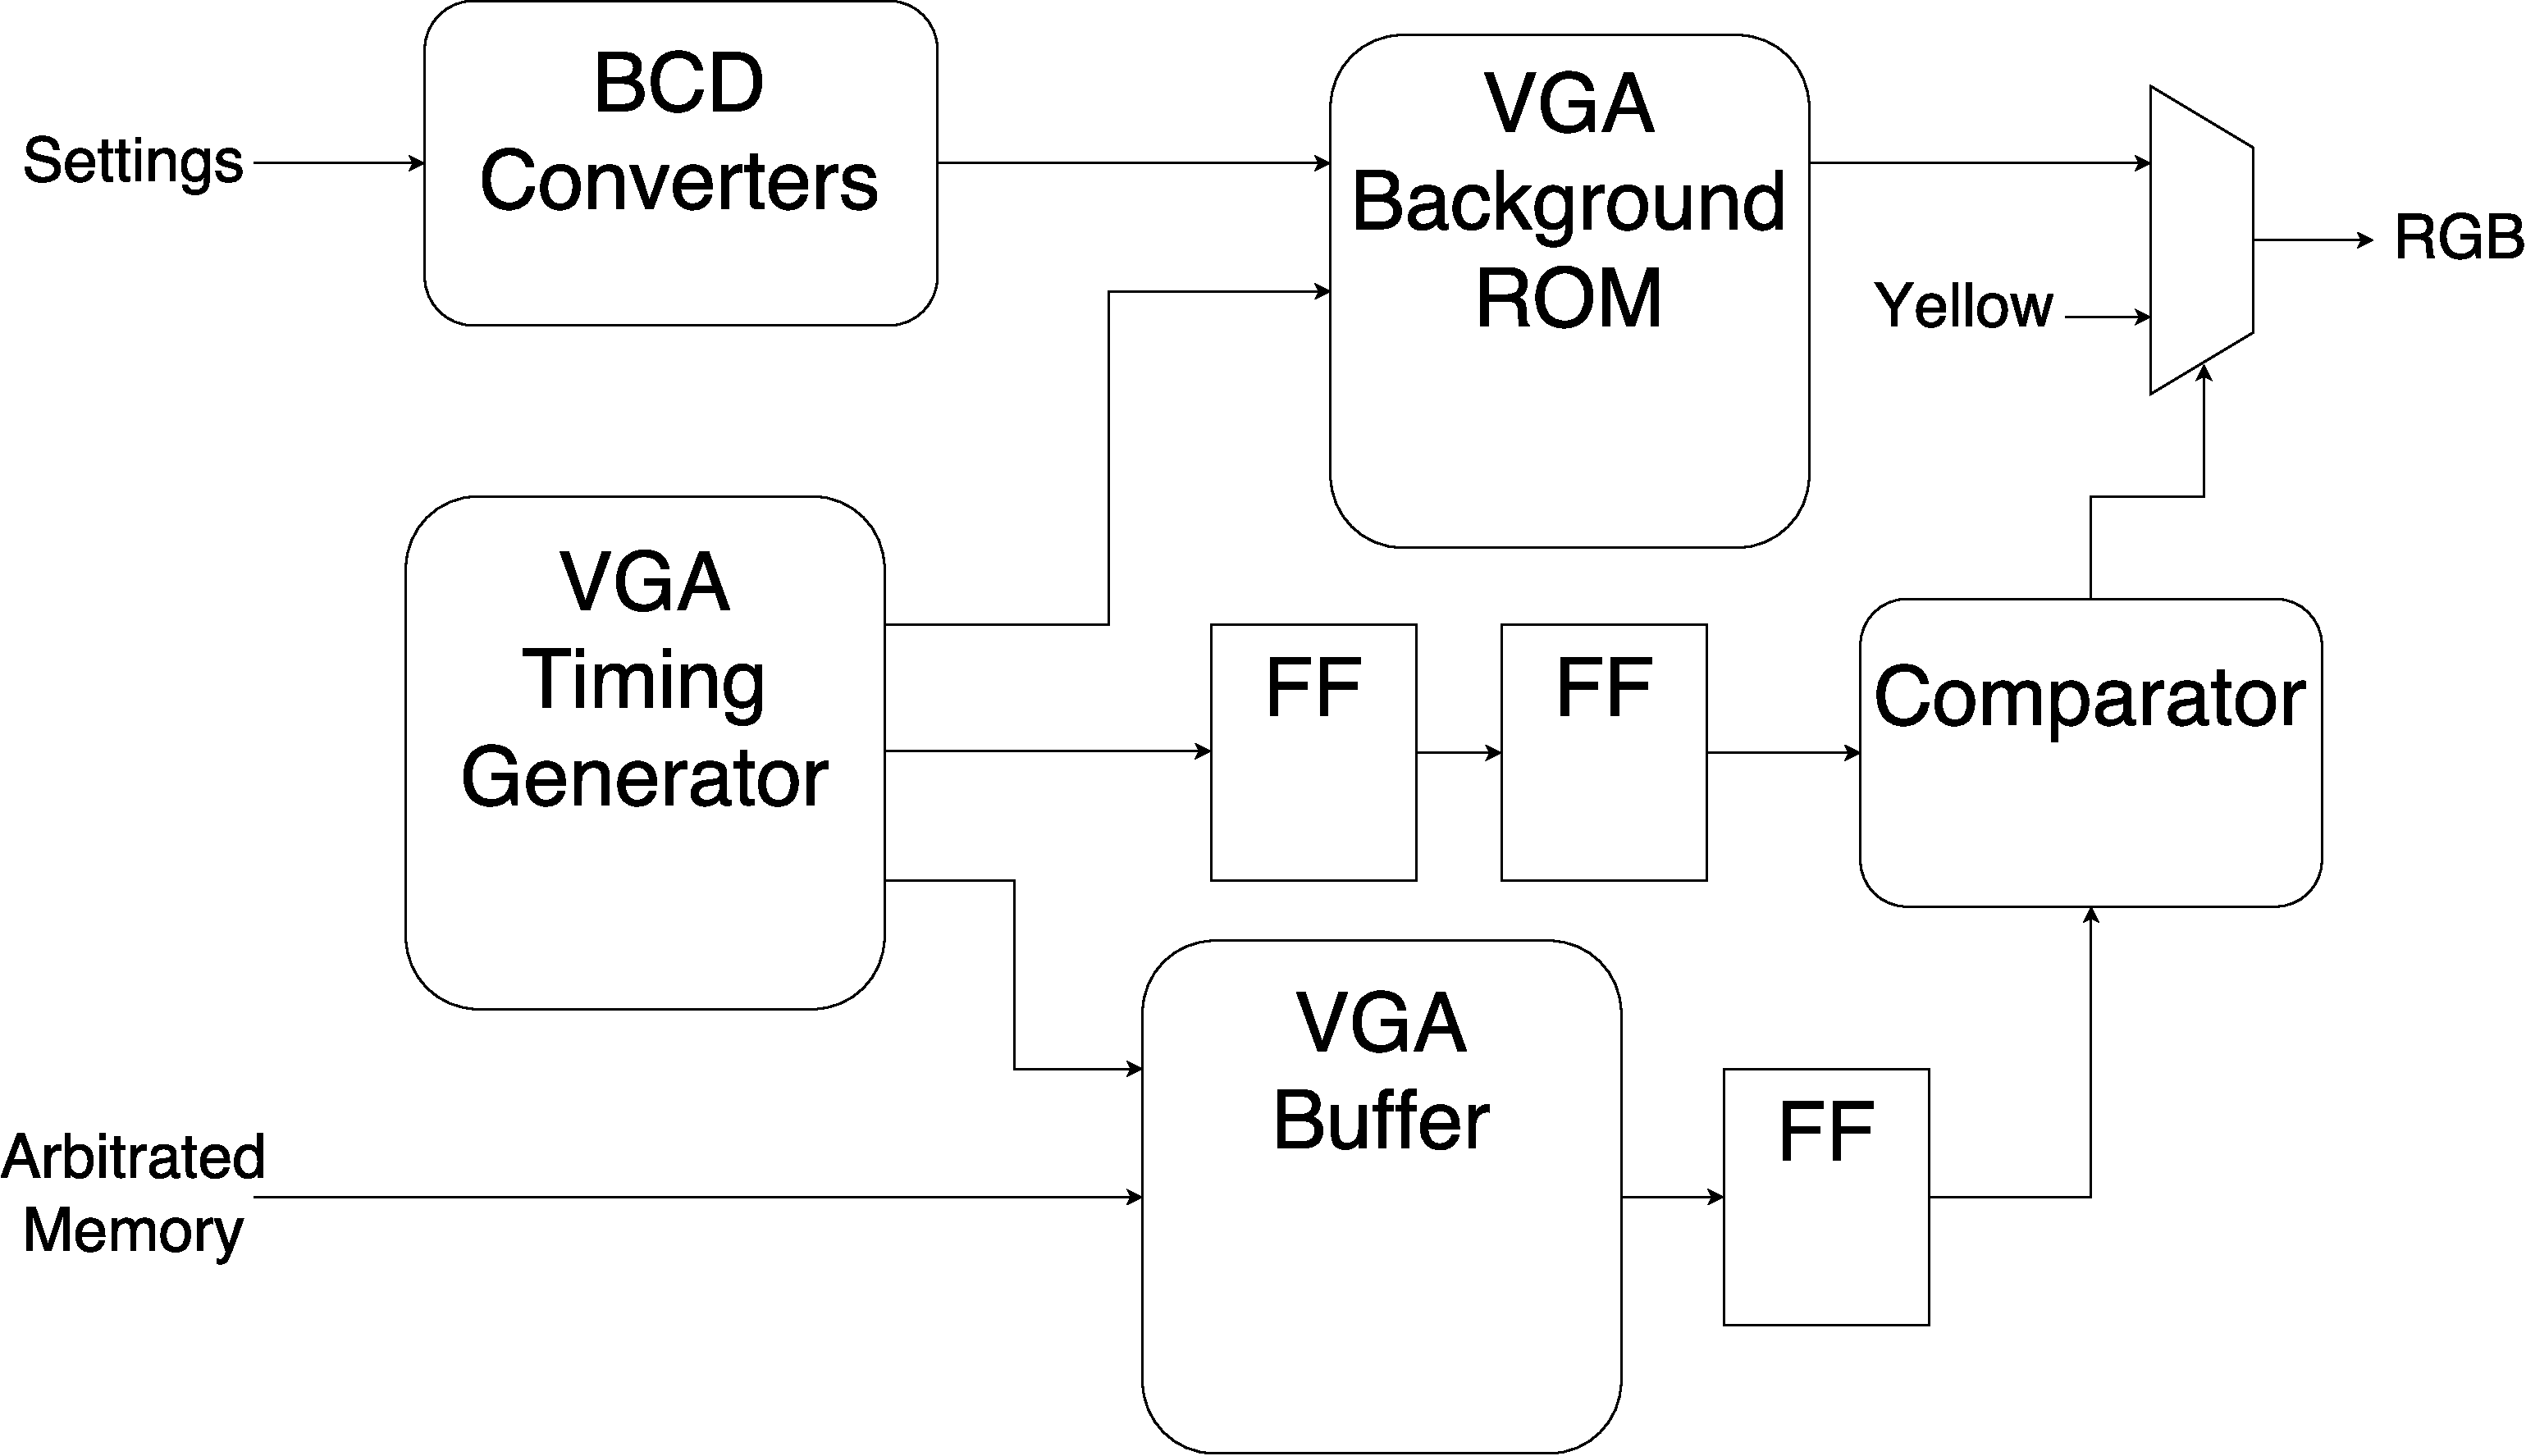
\includegraphics[width=\columnwidth]{diagrams/vga_driver.pdf}
  \caption{Block diagram of the VGA driver module.}
  \label{fig:vga_driver}
\end{figure}

The VGA timing generator entity is used to produce the signals that control the VGA output, such as the VSYNC and HSYNC synchronization signals, the ROW and COLUMN screen position signals, and the BLANK signal for blanking the on-screen data when outside of the visible area.

The VGA buffer entity burst reads the data from the arbitrated memory block when the VSYNC signal goes low. Once completed, it outputs the value of the data for the current COLUMN. In order to allow for vertical interpolation between consecutive data points, it also outputs the subsequent data point. If no such data point exists, it outputs the same data point twice.
These data signals are then passed through a comparator, which determines if the current pixel should be drawn. It does so by checking that the current ROW lies between the two consecutive data points. If it does, it outputs a control signal which sets the output color to yellow for the waveform.

If the current ROW lies outside the consecutive data points, the output color is determined by the VGA background ROM module. This module takes as inputs the VGA timings and the settings and measurements to display on the screen. To allow for conversion between numerical data and ASCII encoding, the measurements and settings are passed through a set of binary-coded decimal (BCD) converters, which convert the numbers into a set of 4-bit decimal digits that can be easily processed. A block diagram of the background ROM module is shown in Figure~\ref{fig:vga_rom}.

\begin{figure}[!htb]
  \centering
  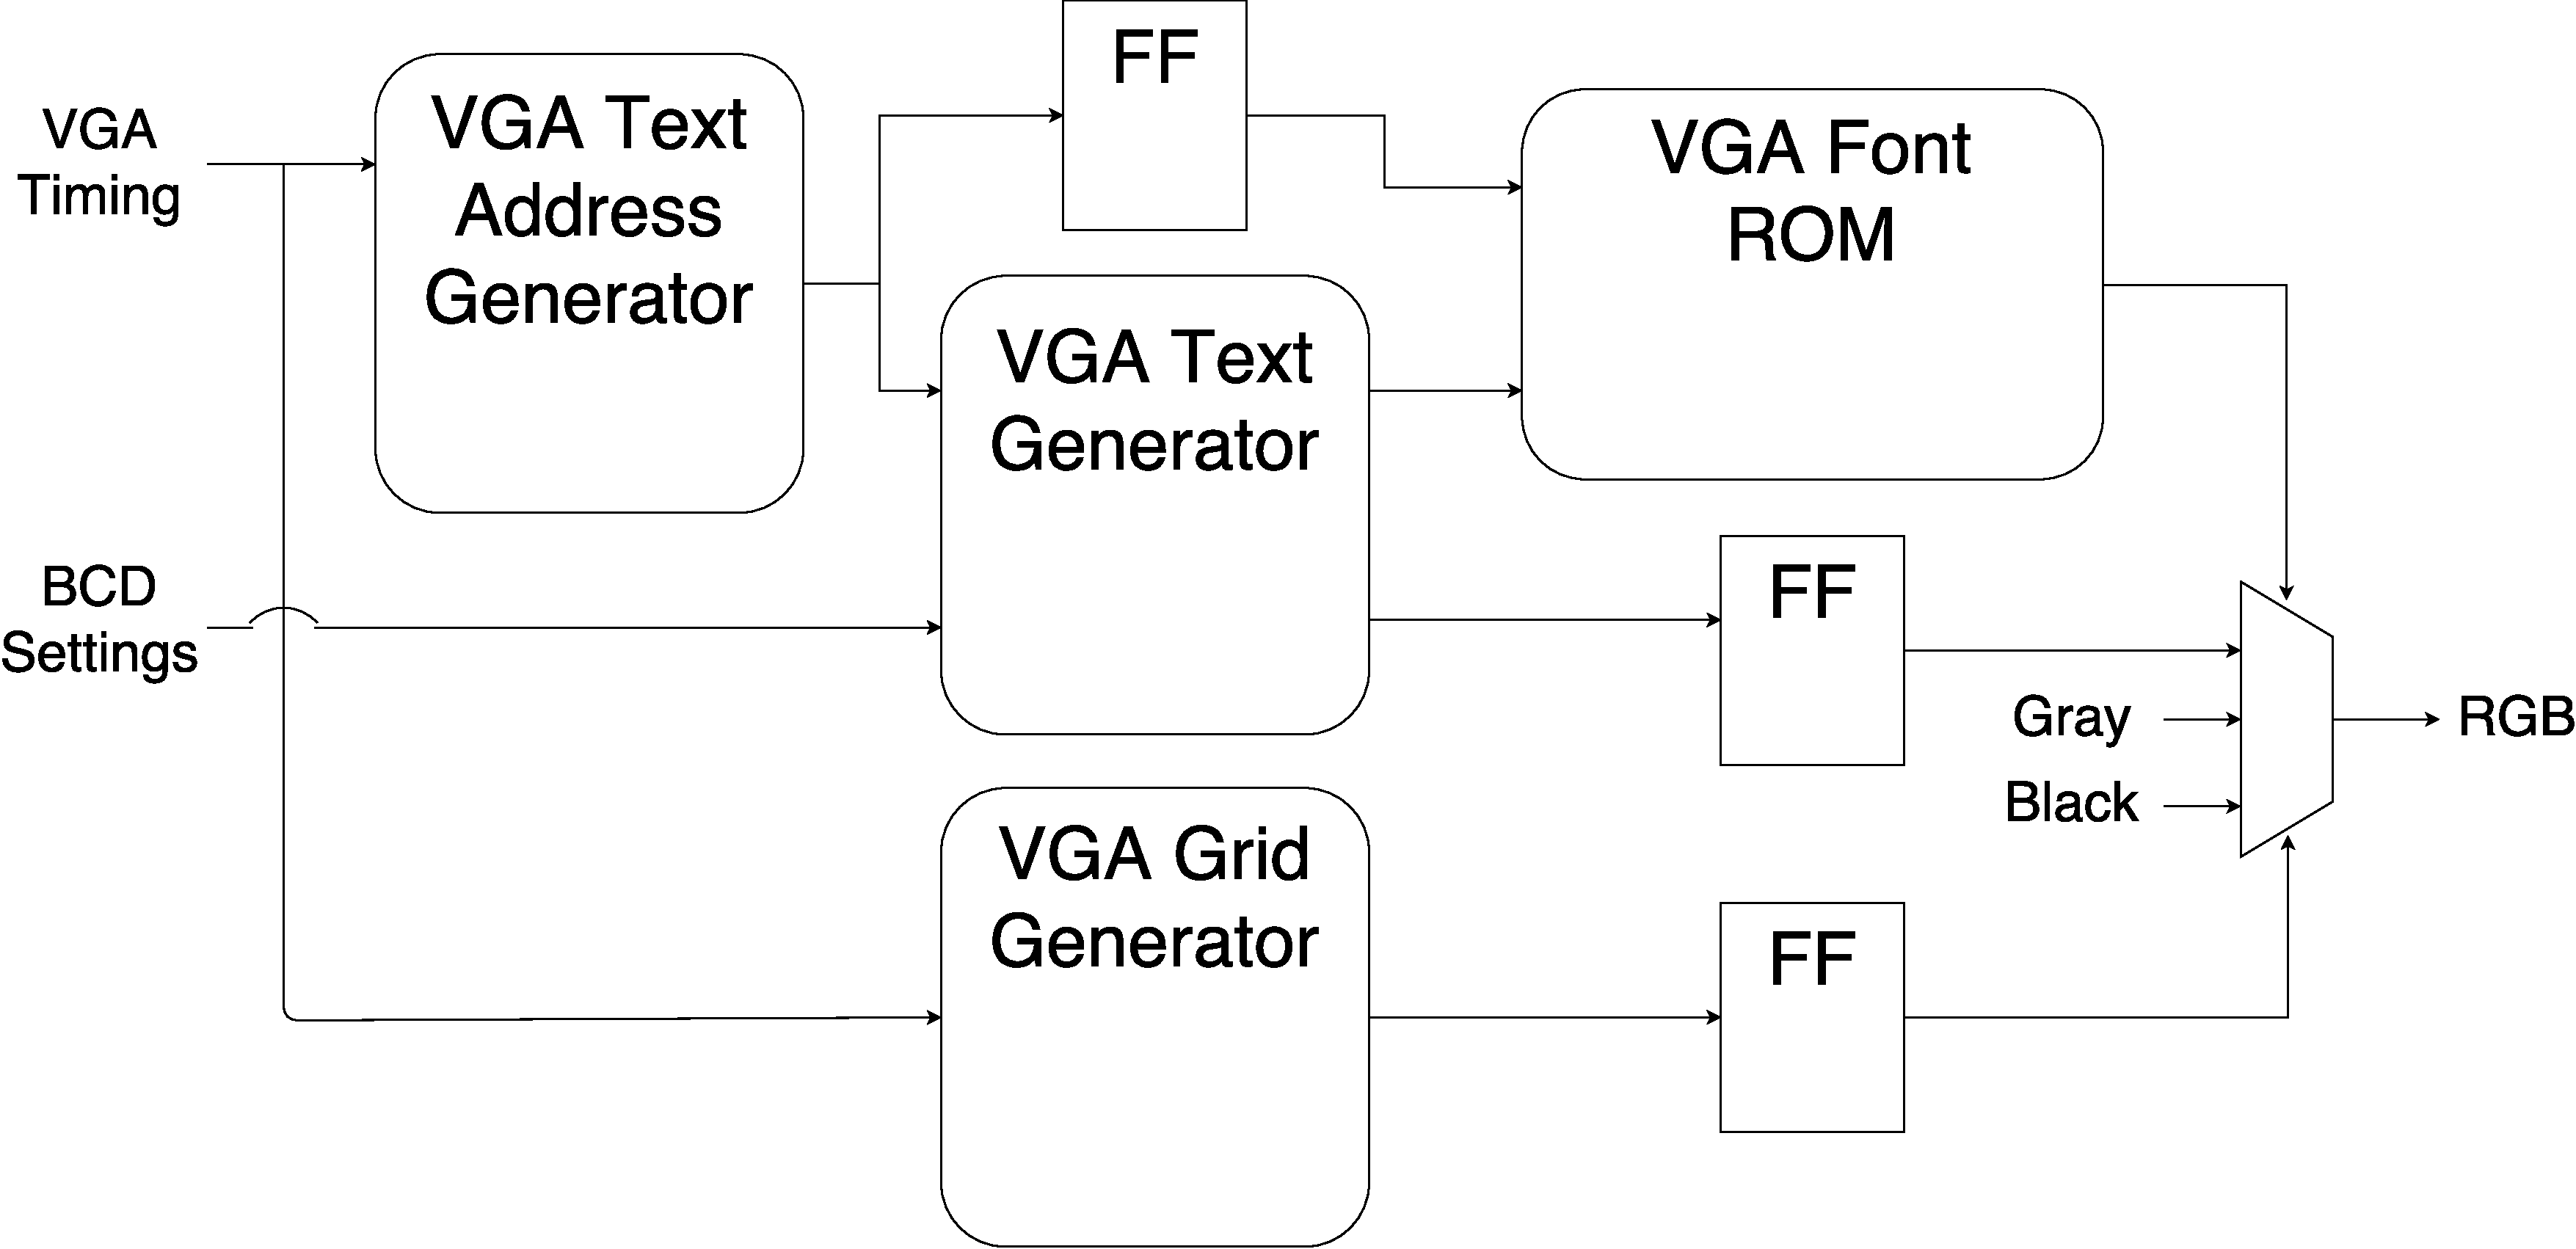
\includegraphics[width=\columnwidth]{diagrams/vga_rom.pdf}
  \caption{Block diagram of the VGA background ROM module.}
  \label{fig:vga_rom}
\end{figure}

To produce the background image, the VGA text address generator entity first converts the ROW and COLUMN values to a new coordinate system better suited to text characters. These coordinates, along with the BCD measurements and settings, are passed to the VGA text generator entity, which determines the character to be drawn at the current position. This character then passes to a VGA font ROM, which determines if the current pixel should be drawn.
In parallel, the VGA grid generator entity checks the current ROW and COLUMN values and determines if the current pixel corresponds to a point on the waveform grid. If it does, it outputs a control signal to color the current pixel in gray.

Throughout this module, registers have been added to equalize the delay paths between signals. These are shown as FF blocks on the diagrams, which stand for flip-flops.

\subsection{Triggering}

Next, we designed the triggering module, which generates a trigger signal in order to achieve a stable waveform display and clear signal characterization. A block diagram of the module can be seen in Figure~\ref{fig:triggering}. The trigger type can be either rising or falling edge, and it controls a comparator which compares the current ADC data, the previous ADC data, and the trigger reference in order to determine if a trigger should occur. For a rising edge trigger type, the previous data should be less than or equal to the reference, and the current data should be greater than the reference. For a falling edge trigger type, the previous data should be greater than or equal to the reference, and the current data should be less than the reference.

\begin{figure}[!htb]
  \centering
  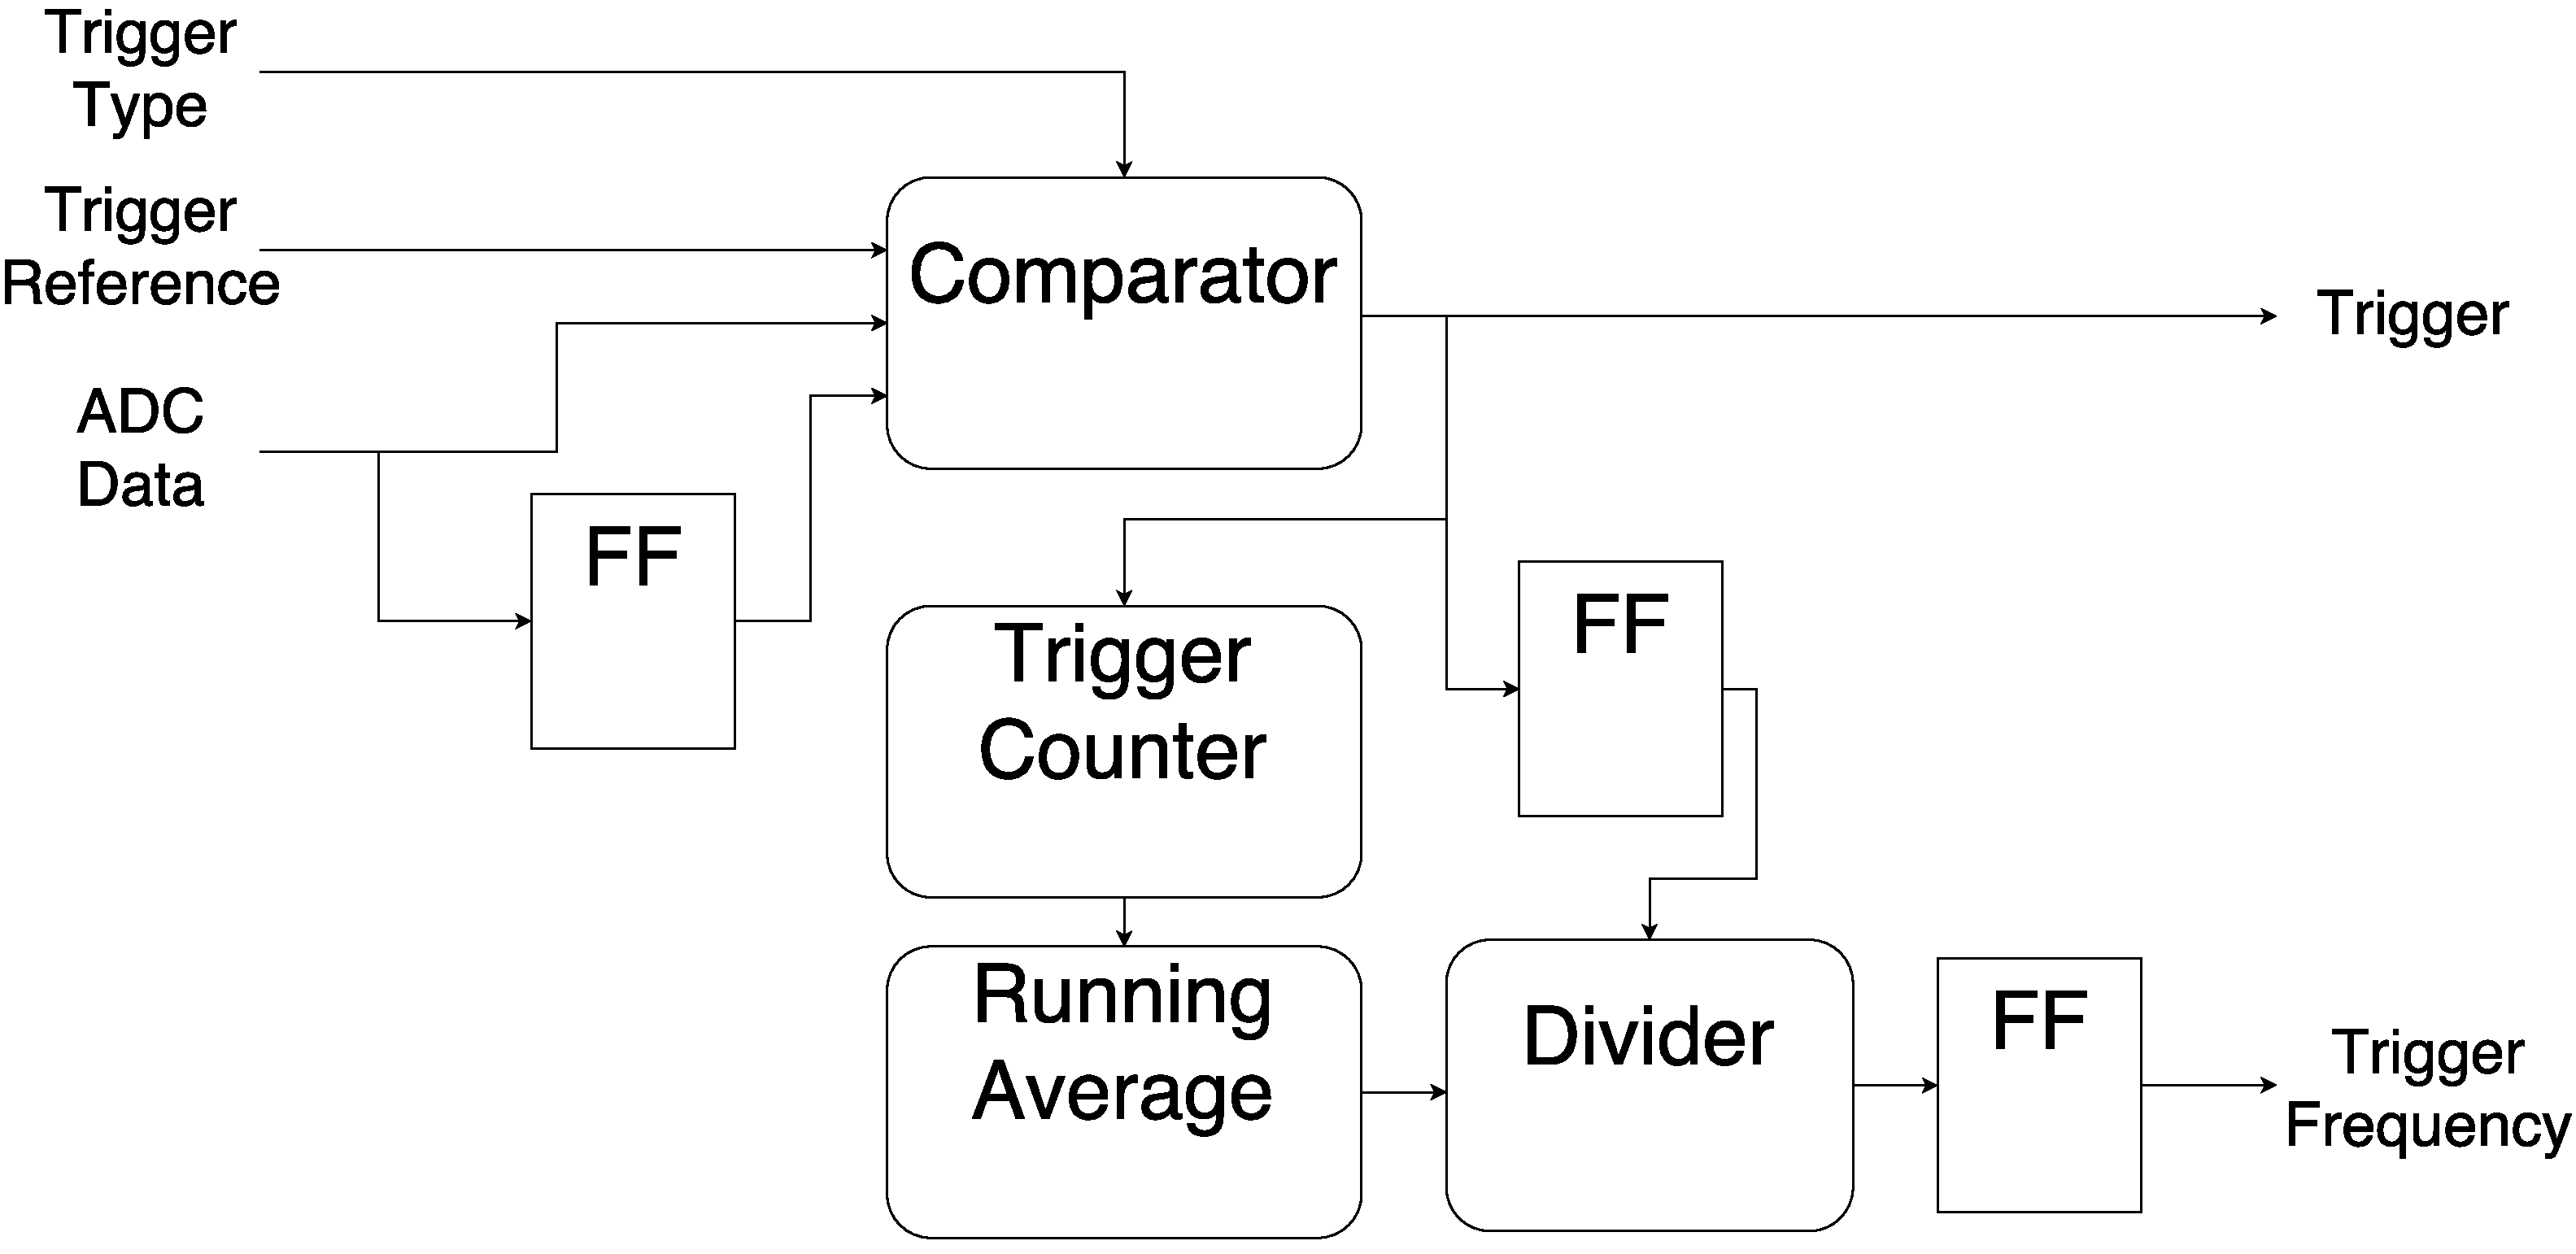
\includegraphics[width=\columnwidth]{diagrams/triggering.pdf}
  \caption{Block diagram of the triggering module.}
  \label{fig:triggering}
\end{figure}

The triggering module also computes and outputs the trigger frequency. It does so through the use of an internal counter which counts the time between trigger signals. The output of this counter is passed through a running average block, which reduces the effect of trigger jitter and outputs the trigger period count. When a trigger occurs, the counter is reset and the running average is enabled in order to save the current trigger period count. A delayed trigger signal then enables a multi-cycle divider which divides the clock rate by the average trigger period count in order to obtain the trigger frequency, which is stored in a register and output. The use of a multi-cycle divider allows us to keep the clock rate high by spreading the latency of a division across multiple clock cycles.

\subsection{Data Acquisition}

We then designed the data acquisition module, which acquires the data sampled by the ADC and writes captured waveforms to an arbitrated memory block when triggered. A block diagram of the module is shown in Figure~\ref{fig:data_acquisition}. The waveform data is stored in an internal RAM block, which is made twice as large as the maximum captured waveform in order to allow the ADC to sample continuously. In order to prevent loss of ADC sample points, we give full priority to the ADC in terms of access to this RAM block. The ADC enable signal increments the ADC address and writes the current sample point to the RAM by controlling an address multiplexer.

\begin{figure}[!htb]
  \centering
  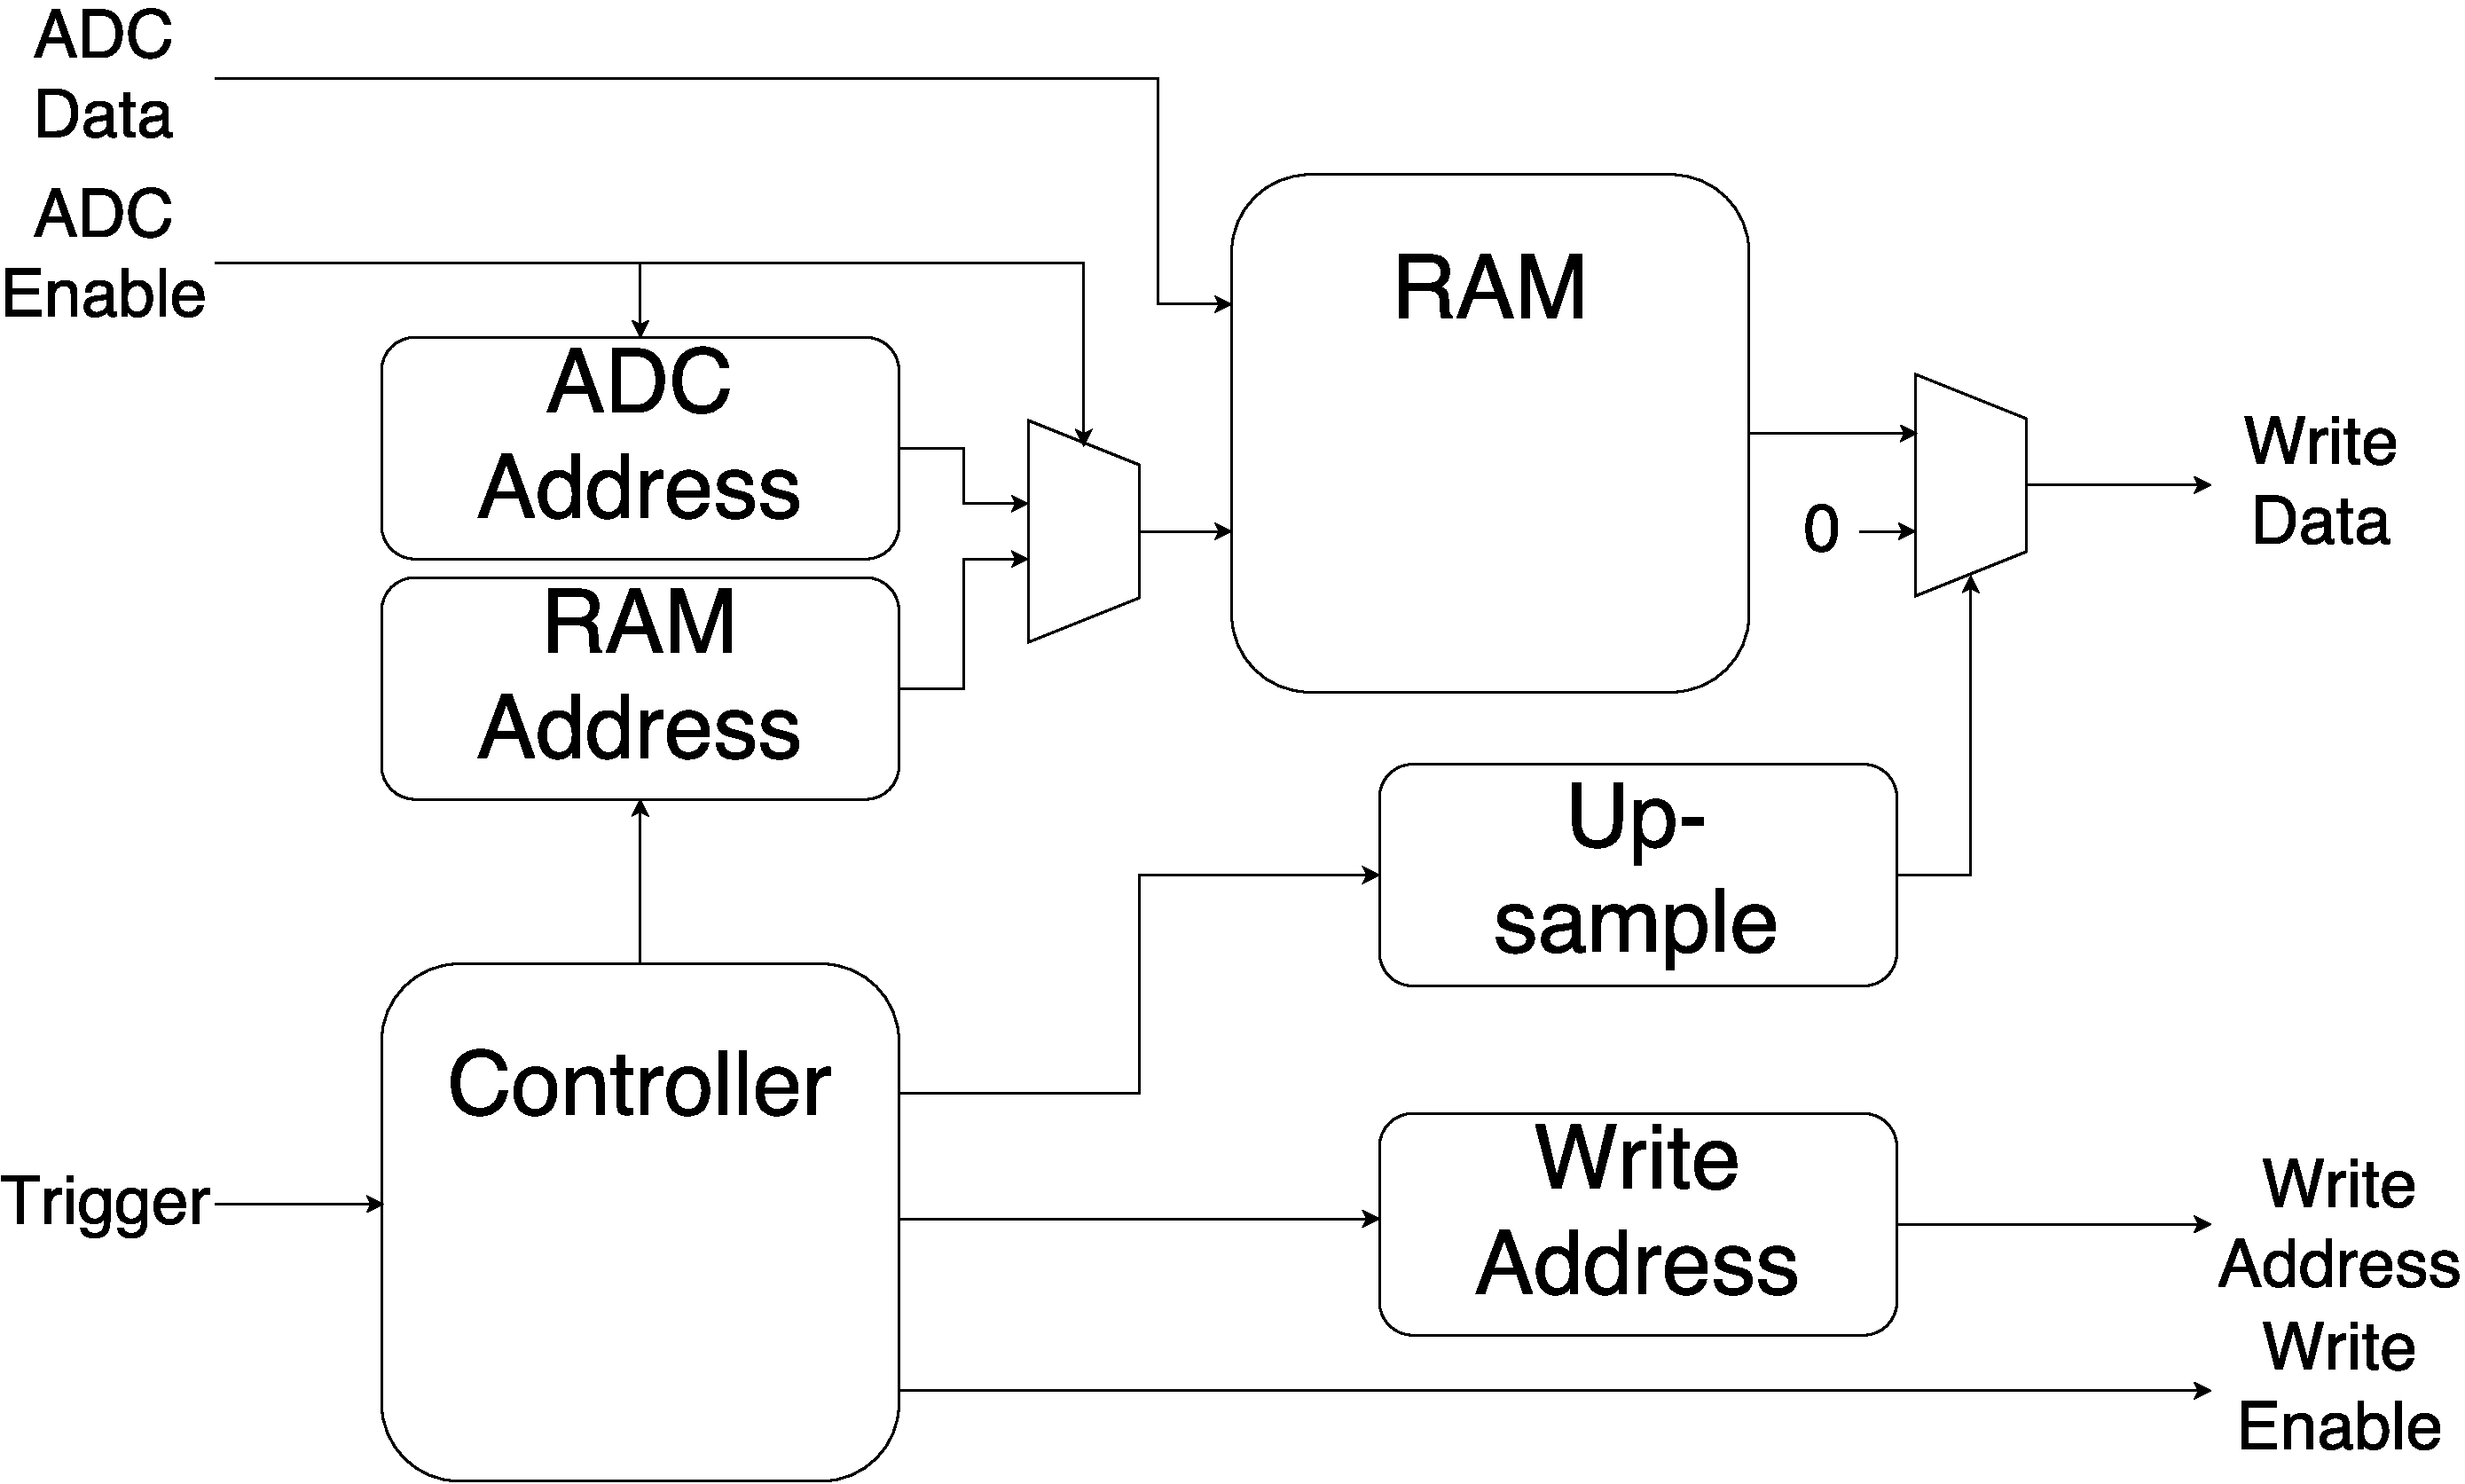
\includegraphics[width=\columnwidth]{diagrams/data_acquisition.pdf}
  \caption{Block diagram of the data acquisition module.}
  \label{fig:data_acquisition}
\end{figure}

The rest of the module consists of the waveform capture blocks. A finite state machine controller waits for a trigger signal to start. Once triggered, it counts the number of points sampled by the ADC until it determines that it has enough data to capture a waveform with the trigger point in the center. It then outputs signals to control the RAM address and write address counters in order to read data from the RAM and output it to an arbitrated memory block.

This controller is also in charge of up-sampling the data. It uses an up-sample counter to output zeros between sample points, according to the current horizontal time scale setting. This allows subsequent modules to interpolate the data at these up-sampled points, and has the effect of zooming in on the waveform.

\subsection{Sin(x)/x Interpolation}

The interpolation module is currently being implemented.

\subsection{Voltage Measurements}

The voltage measurement modules are currently being implemented.

\section{Results}

In order to ensure proper functioning, every module was tested independently before being combined with other modules to form the system. Most of these tests consisted of checking the outputs of a module against the expected outputs for a set of specified inputs, and these tests were automated to produce a single error count, saving us the trouble of checking timing diagrams manually. We therefore describe only the most relevant results here.

First, to test the VGA timings, we created a test-bench which would output a simple array of color bars to the screen. The test-bench was made to log the VGA signals at each clock cycle to a file, which we could then view on a VGA simulator. The resulting screen capture is shown in Figure~\ref{fig:vga_timing_test}.

\begin{figure}[!htb]
  \centering
  
\includegraphics[width=\columnwidth]{test-results/vga_timing.png}
  \caption{VGA timing test results.}
  \label{fig:vga_timing_test}
\end{figure}

Then, we tested the entire VGA module by creating a test-bench which connected an arbitrated memory block to the input of the VGA driver. We loaded several test signals in this memory block before the simulation, and logged the resulting VGA signals to a text file. We used a simulator to view the resulting display, and the results are shown in Figures~\ref{fig:vga_test_1}~and~\ref{fig:vga_test_2}. Note that the displayed data is for illustration purposes only and does not correspond to real measurements.

\begin{figure}[!htb]
  \centering
  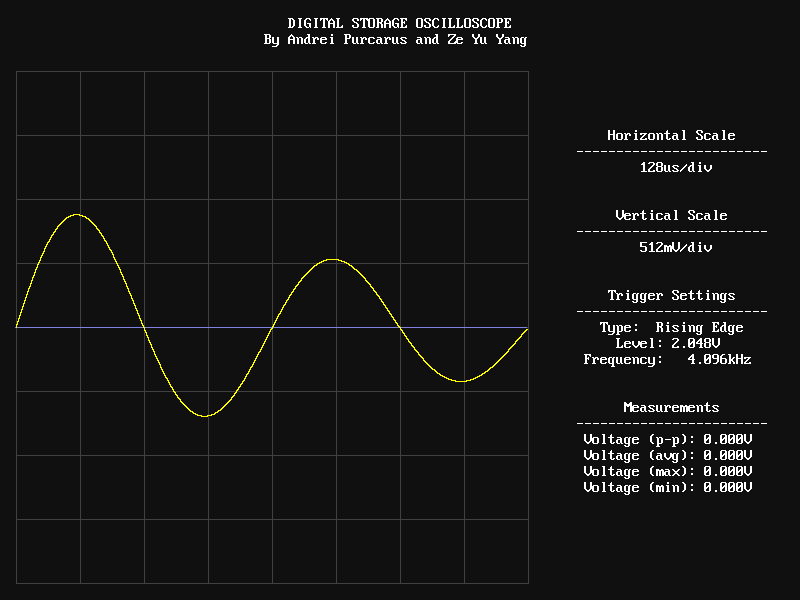
\includegraphics[width=\columnwidth]{test-results/vga_test_signal1.png}
  \caption{VGA driver test results for an exponentially decaying sine wave signal.}
  \label{fig:vga_test_1}
\end{figure}

\begin{figure}[!htb]
  \centering
  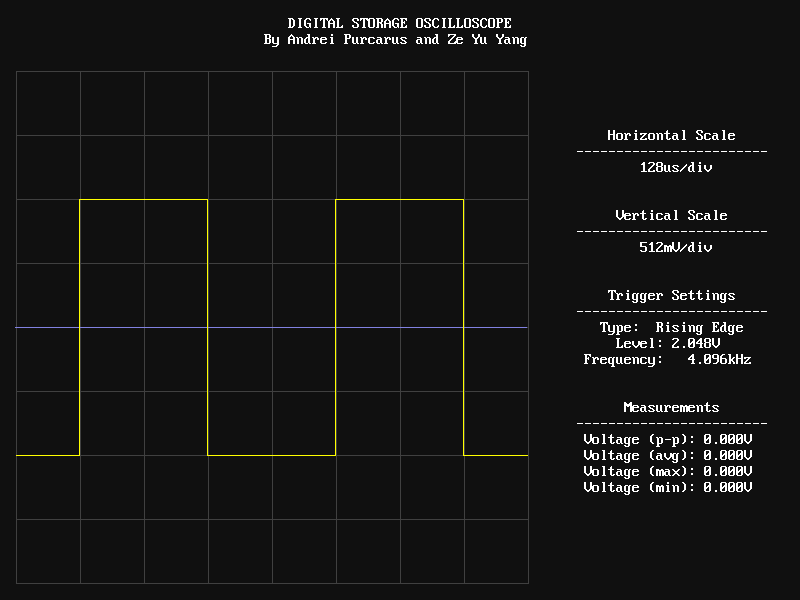
\includegraphics[width=\columnwidth]{test-results/vga_test_signal2.png}
  \caption{VGA driver test results for a square wave signal.}
  \label{fig:vga_test_2}
\end{figure}

Next, we tested the triggering module. We connected the analog waveform generator module we created in a previous assignment to the input of the triggering module and observed the resulting signals. The resulting timing diagrams are shown in Figures~\ref{fig:trigger_test_1}~and~\ref{fig:trigger_test_2}. From these diagrams, we can see that the module triggers correctly on both falling and rising edges, and that the frequency is correctly identified, with an error of 0.04~\% for the 10~kHz signal and 0.00~\% for the 200~kHz signal.

\begin{figure}[!htb]
  \centering
  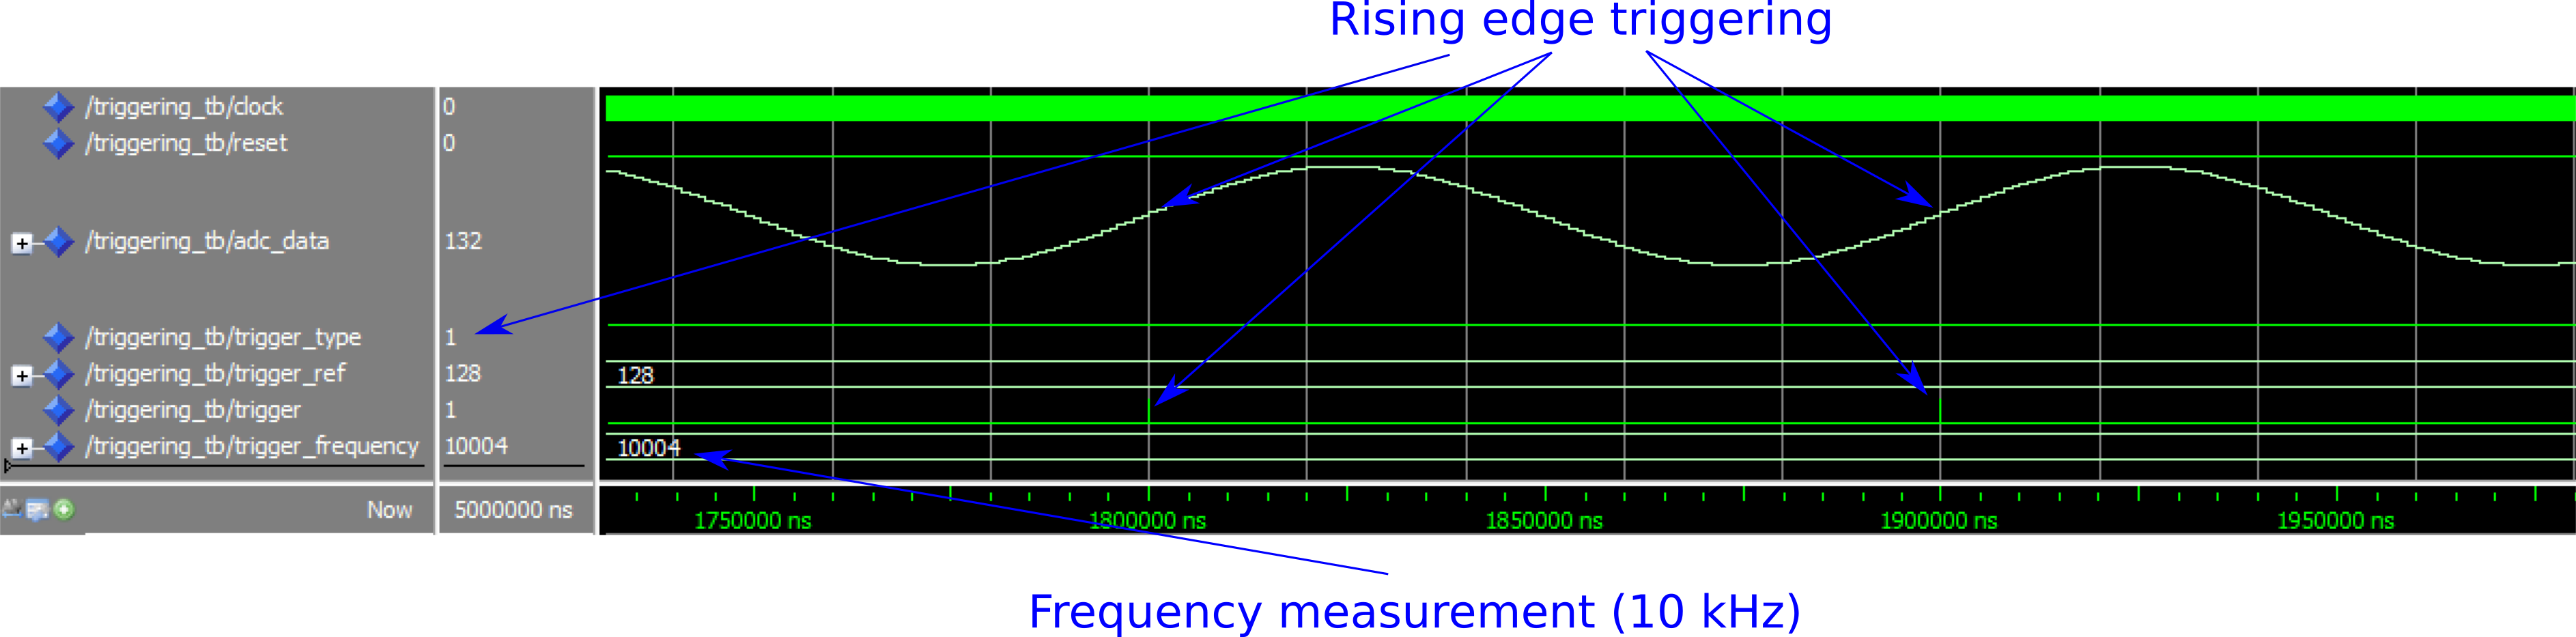
\includegraphics[width=\columnwidth]{test-results/trigger_test_rising_10kHz.png}
  \caption{Triggering test results for a rising edge trigger type on a 10~kHz sine wave.}
  \label{fig:trigger_test_1}
\end{figure}

\begin{figure}[!htb]
  \centering
  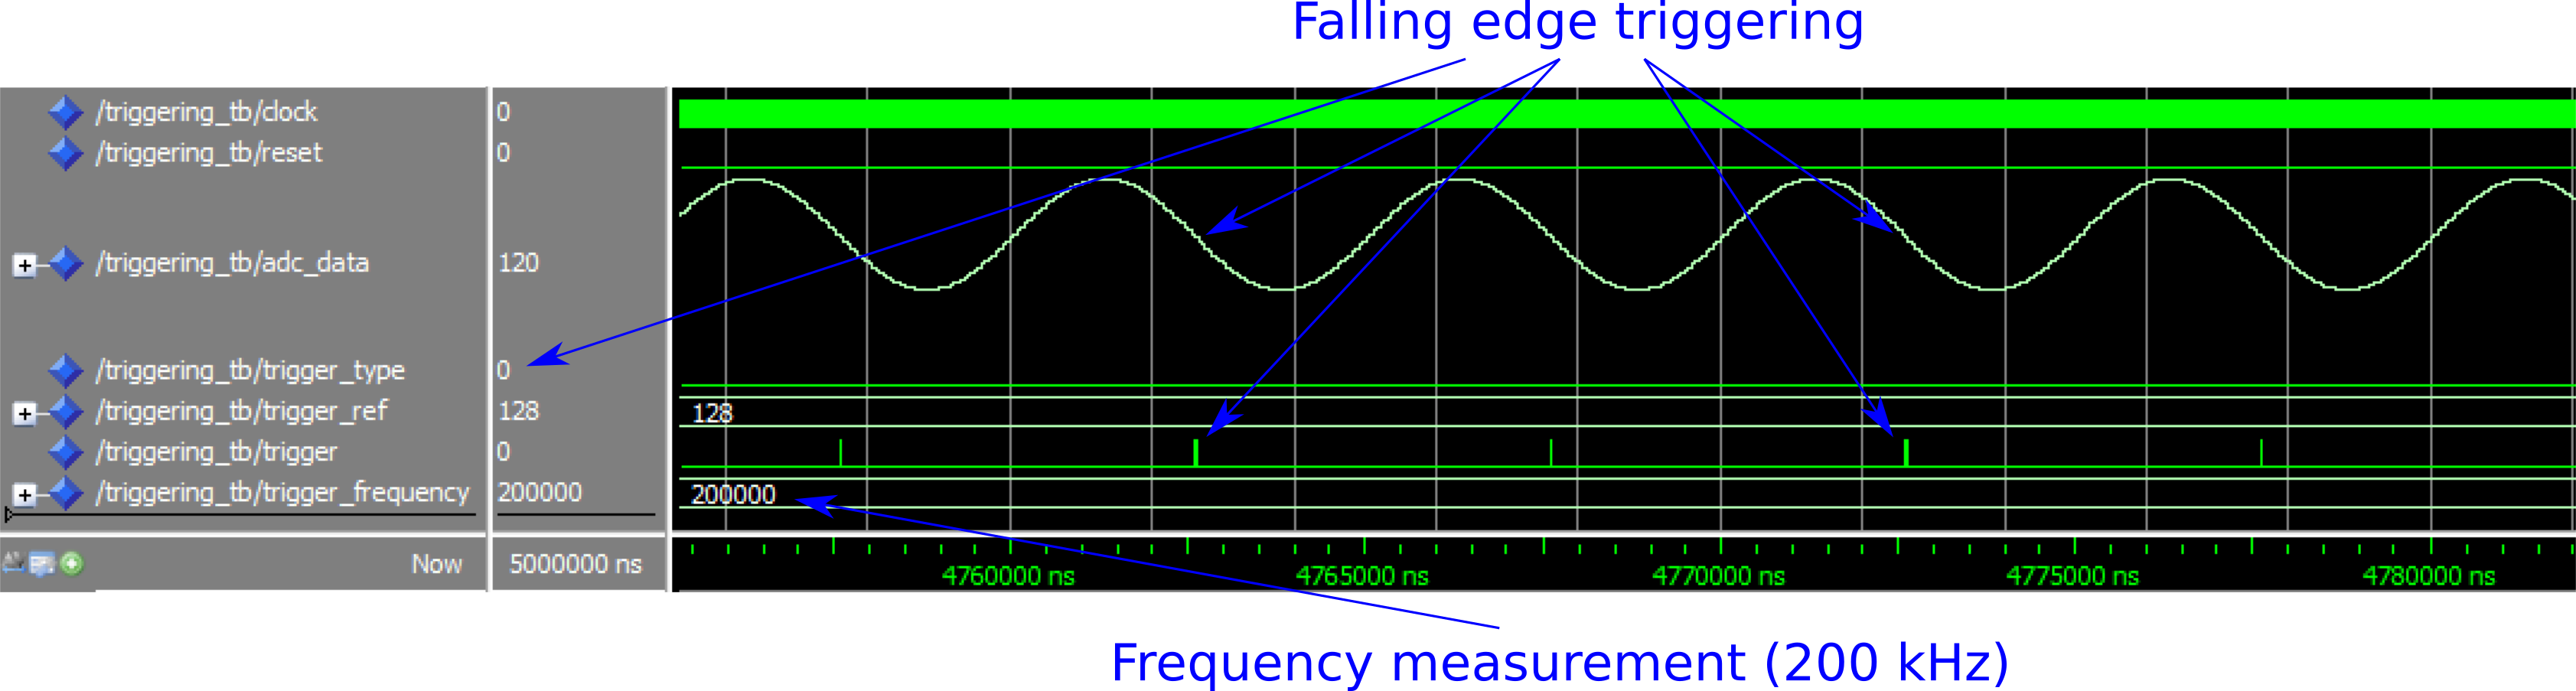
\includegraphics[width=\columnwidth]{test-results/trigger_test_falling_200kHz.png}
  \caption{Triggering test results for a falling edge trigger type on a 200~kHz sine wave.}
  \label{fig:trigger_test_2}
\end{figure}

We then tested the data acquisition module by connecting the triggering and analog waveform generator modules as inputs and observing the state transitions of the internal controller. The results are shown in Figure~\ref{fig:data_acq_test}. From this figure, we can see that the controller switches into a triggered state when a trigger occurs, and waits for sufficient sampled data to be available before burst writing the waveform to memory.

\begin{figure}[!htb]
  \centering
  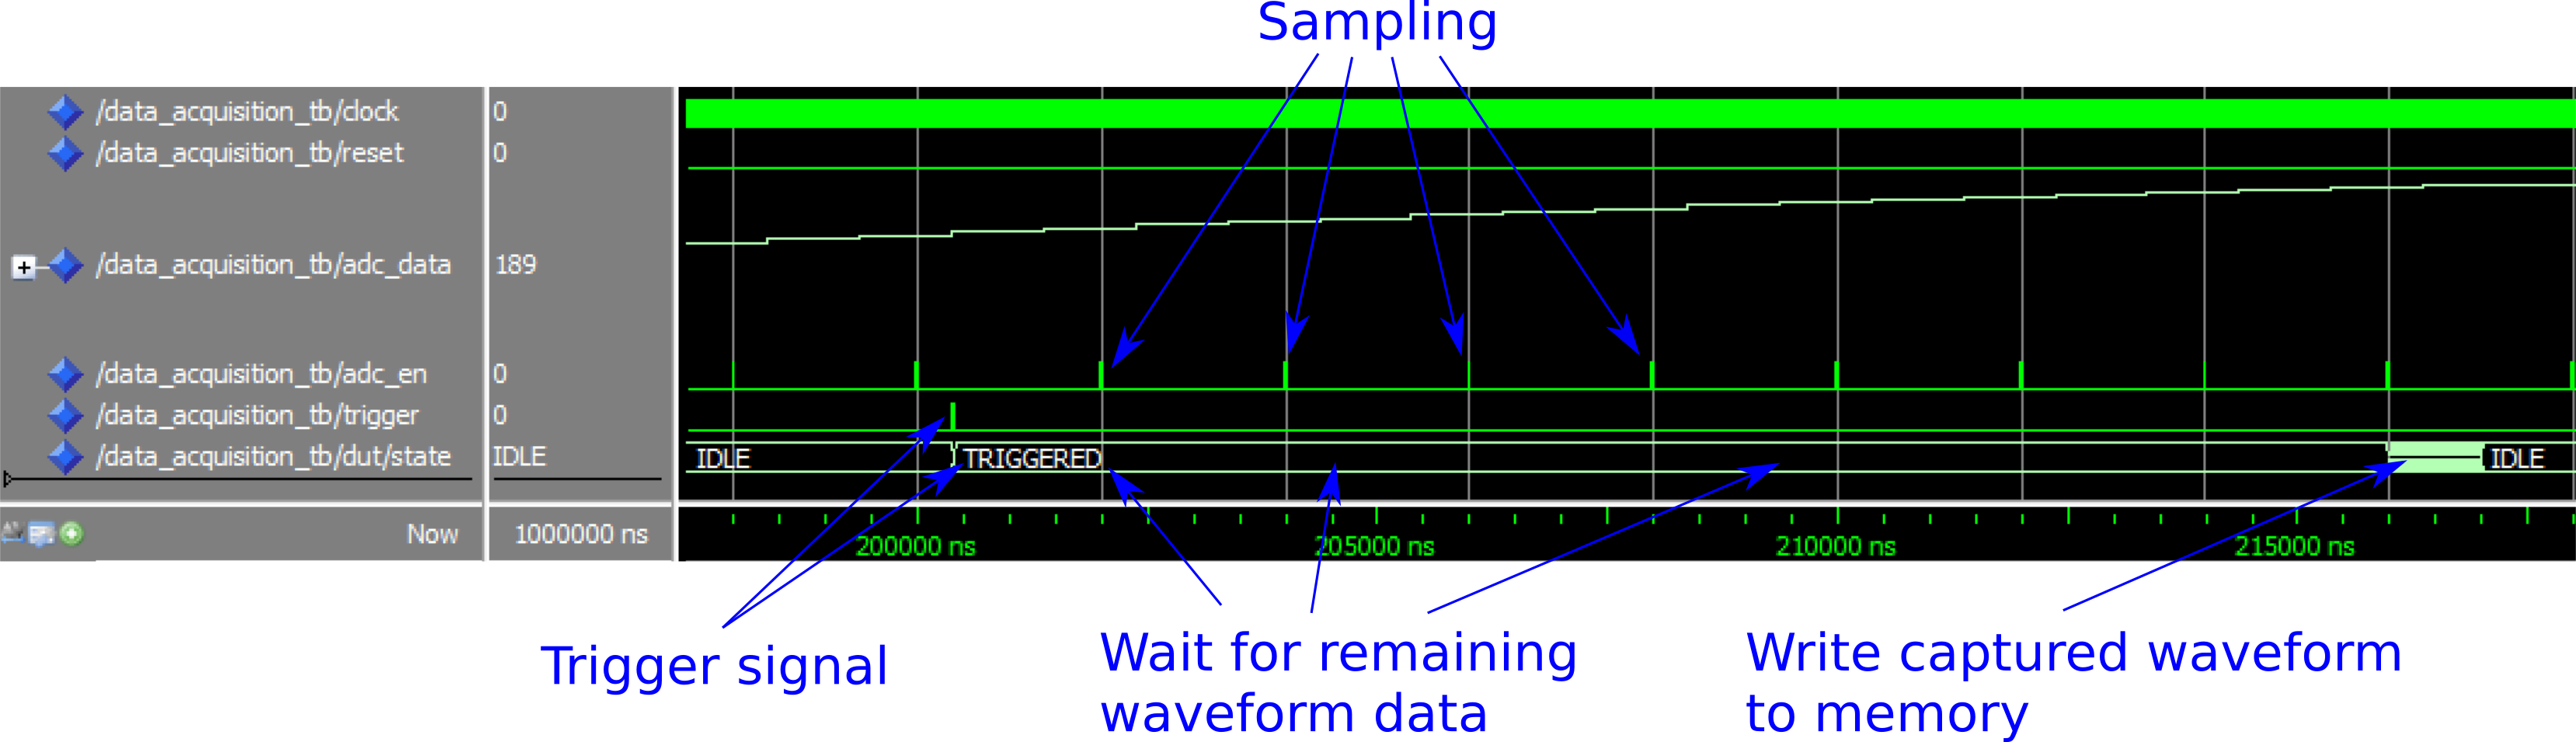
\includegraphics[width=\columnwidth]{test-results/data_acquisition_test.png}
  \caption{Data acquisition test results.}
  \label{fig:data_acq_test}
\end{figure}

Next, we combined all the modules together into a top level DSO entity. Since interpolation was not yet ready, we connected the first arbitrated memory block from Figure~\ref{fig:system} to both the data acquisition module and the VGA driver module. We then connected the analog waveform generator as an input to the system and observed the resulting VGA outputs for different signal frequencies. The results are shown in Figures~\ref{fig:scope_test_1},~\ref{fig:scope_test_2},~\ref{fig:scope_test_3},~and~\ref{fig:scope_test_4}. Note that the timebase was changed for the different frequencies to show the effects of up-sampling. We can see from these figures that the sample points are correctly displayed, and the frequencies are correctly computed, with errors of 0.10~\%, 0.04~\%, 0.00~\%, and 0.00~\% for frequencies of 1~kHz, 10~kHz, 100~kHz, and 200~kHz, respectively.

In addition, we can see the effects of up-sampling on a captured waveform, in particular for the 200~kHz waveform in Figure~\ref{fig:scope_test_4}, which is barely identifiable as a sine wave. We will see the effects of interpolation in the reconstruction of these waveforms when the interpolation module is completed.

\begin{figure}[!htb]
  \centering
  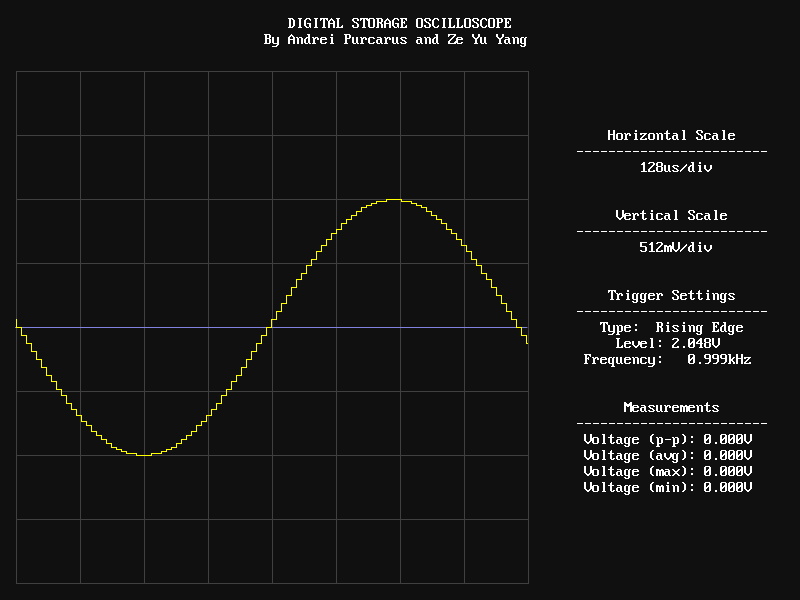
\includegraphics[width=\columnwidth]{test-results/scope_demo_1kHz.png}
  \caption{Oscilloscope test results for a 1~kHz sine wave input on a 128~us/div horizontal scale.}
  \label{fig:scope_test_1}
\end{figure}

\begin{figure}[!htb]
  \centering
  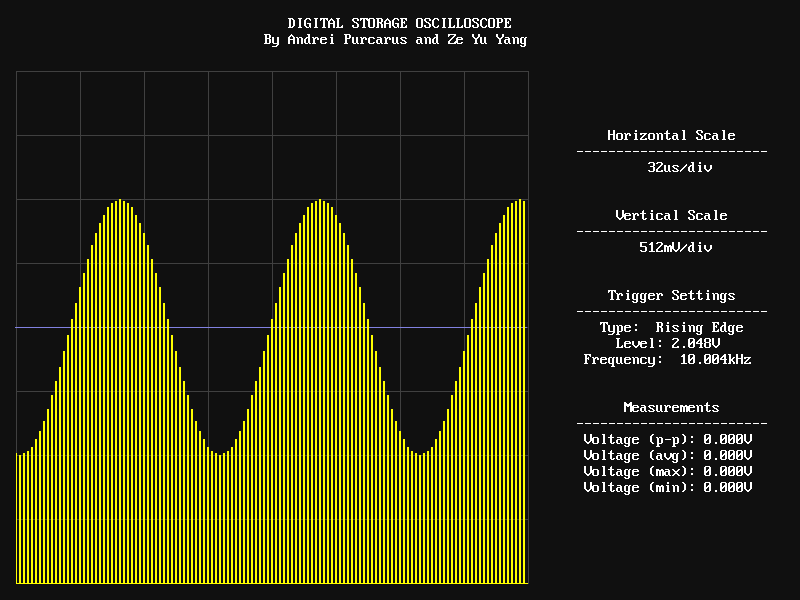
\includegraphics[width=\columnwidth]{test-results/scope_demo_10kHz.png}
  \caption{Oscilloscope test results for a 10~kHz sine wave input on a 32~us/div horizontal scale.}
  \label{fig:scope_test_2}
\end{figure}

\begin{figure}[!htb]
  \centering
  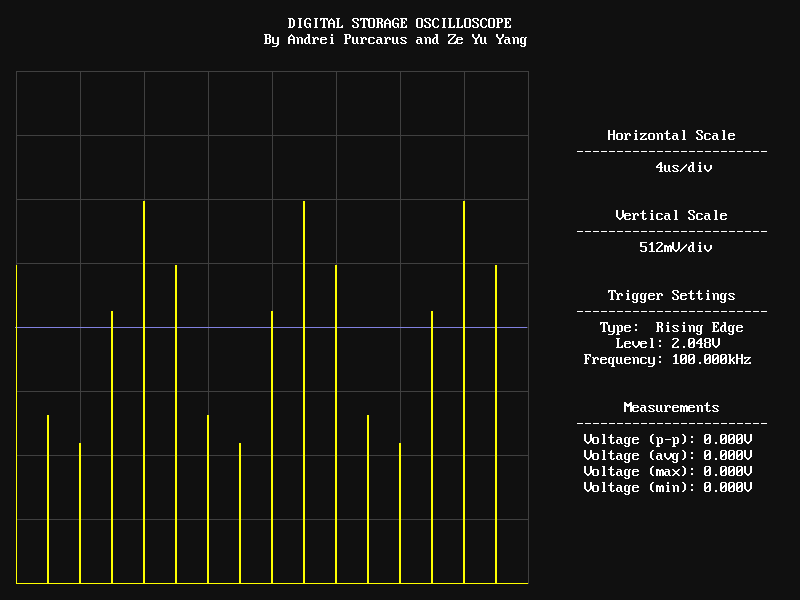
\includegraphics[width=\columnwidth]{test-results/scope_demo_100kHz.png}
  \caption{Oscilloscope test results for a 100~kHz sine wave input on a 4~us/div horizontal scale.}
  \label{fig:scope_test_3}
\end{figure}

\begin{figure}[!htb]
  \centering
  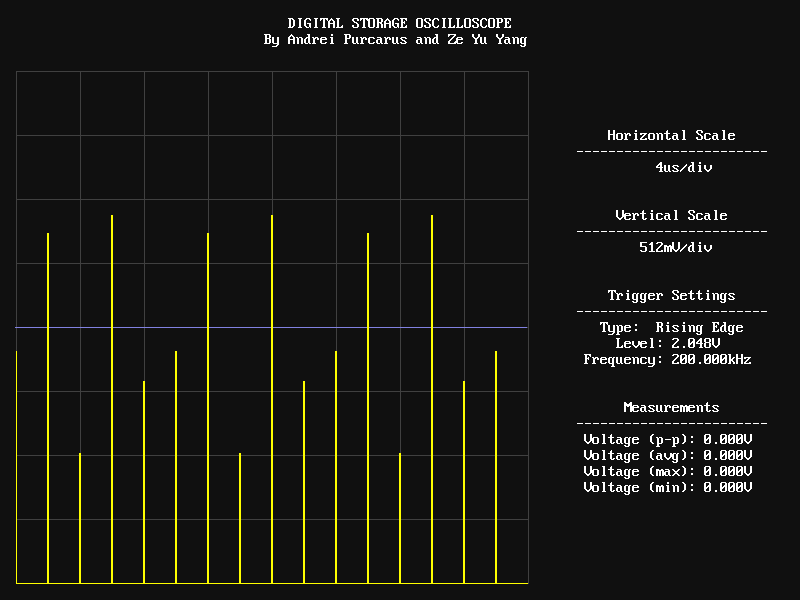
\includegraphics[width=\columnwidth]{test-results/scope_demo_200kHz.png}
  \caption{Oscilloscope test results for a 200~kHz sine wave input on a 4~us/div horizontal scale.}
  \label{fig:scope_test_4}
\end{figure}

We then synthesized the design for the target FPGA. The synthesis results are shown in Table~\ref{tab:synthesis_results}, which shows a maximum clock frequency of 70.83~MHz. This meets our goal of a 50~MHz clock.

\begin{table}[!htb]
    \centering
    \caption{Synthesis results on the Cyclone V 5CSEMA5F31C6 FPGA using a 50~MHz clock.}
    \label{tab:synthesis_results}
    \begin{tabular}[c]{ | l | l | }
    	\hline
        \textbf{Family} & Cyclone V \\
        \hline
        \textbf{Device} & 5CSEMA5F31C6 \\
        \hline
        \textbf{Logic Utilization} & 3,381 / 32,070 ( 11~\% ) \\
        \hline
        \textbf{Total Registers} & 5512 \\
        \hline
        \textbf{Total Block Memory Bits} & 15,136 / 4,065,280 ( $<$~1~\% ) \\
        \hline
        \textbf{Total DSP Blocks} & 0 / 87 ( 0~\% ) \\
        \hline
        \textbf{Fmax} & 70.83~MHz \\
        \hline
        \textbf{Setup Slack} & 5.881~ns \\
        \hline
        \textbf{Hold Slack} & 0.089~ns \\
        \hline
    \end{tabular}
\end{table}

\section{Analysis}

From the results, we can see that our goals are currently being met. The frequency measurements are well within our target accuracy of 1~\%~+~10~Hz. However, these measurements were performed on digital waveforms produced by our analog waveform generator. It remains to be seen how the system will perform for real analog waveforms.

Due to the lack of an interpolation module, we could not evaluate the display of waveforms over the entire frequency range.
Also, due to the lack of voltage measurement modules, we could not evaluate the accuracy of voltage measurements.
Both of these issues will be fixed when these modules are implemented.

From the synthesis results, we can see that our project has been well designed. The use of multi-cycle dividers and BCD converters has allowed us to maintain a high clock frequency while preserving the proper functioning of our DSO. In addition, the low resource usage shows that we still have space to implement the additional modules on the FPGA.

\section{Conclusions}

We implemented most of the modules required for an FPGA implementation of a digital storage oscilloscope. The current implementation is capable of triggering on a waveform, capturing it and displaying it to a VGA monitor. It measures the trigger frequency, a proxy for the frequency of the waveform, with a maximum error of 0.10~\% over the entire target frequency range.

However, the missing interpolation and voltage measurement modules have made it impossible to evaluate our DSO in terms of our other goals. We are currently working on implementing this missing functionality for a proper assessment of our project.

In addition, the tests performed have all been using simulated waveforms. For a proper evaluation of the project, we will synthesize the system on our target FPGA and capture real analog waveforms. We are currently working on writing an interface to the ADC on the DE1-SoC development board to enable these tests. These tests should present a more thorough evaluation of our design due to the presence of noise on signals, which can cause issues such as false triggering and trigger jitter.

\bibliographystyle{IEEEtran}
\bibliography{IEEEabrv,references}

\end{document}
